\section{Analysis and prediction of seiyuu popularity}

\PARstart{P}{opularity} is an abstract criterion that must be defined as a numerical metric in order to be used for analysis and prediction. Since we are using MAL database for seiyuu and anime information and it has a social component; seems logic to use member\_favorites as a representation of popularity. We can also get popularity and score for works from opinions of the same set of users.

In terms of distribution \textit{popularity} is highly unequal \---as we can observe in Fig.~\ref{fig:popularityDistribution}\--- having a lot of seiyuu which are no member favourites and only a few who are favorite of more than 10000 members. It's good to keep in mind that users can favorite multiple seiyuu.

\begin{figure}[!hbt]
	\begin{center}
	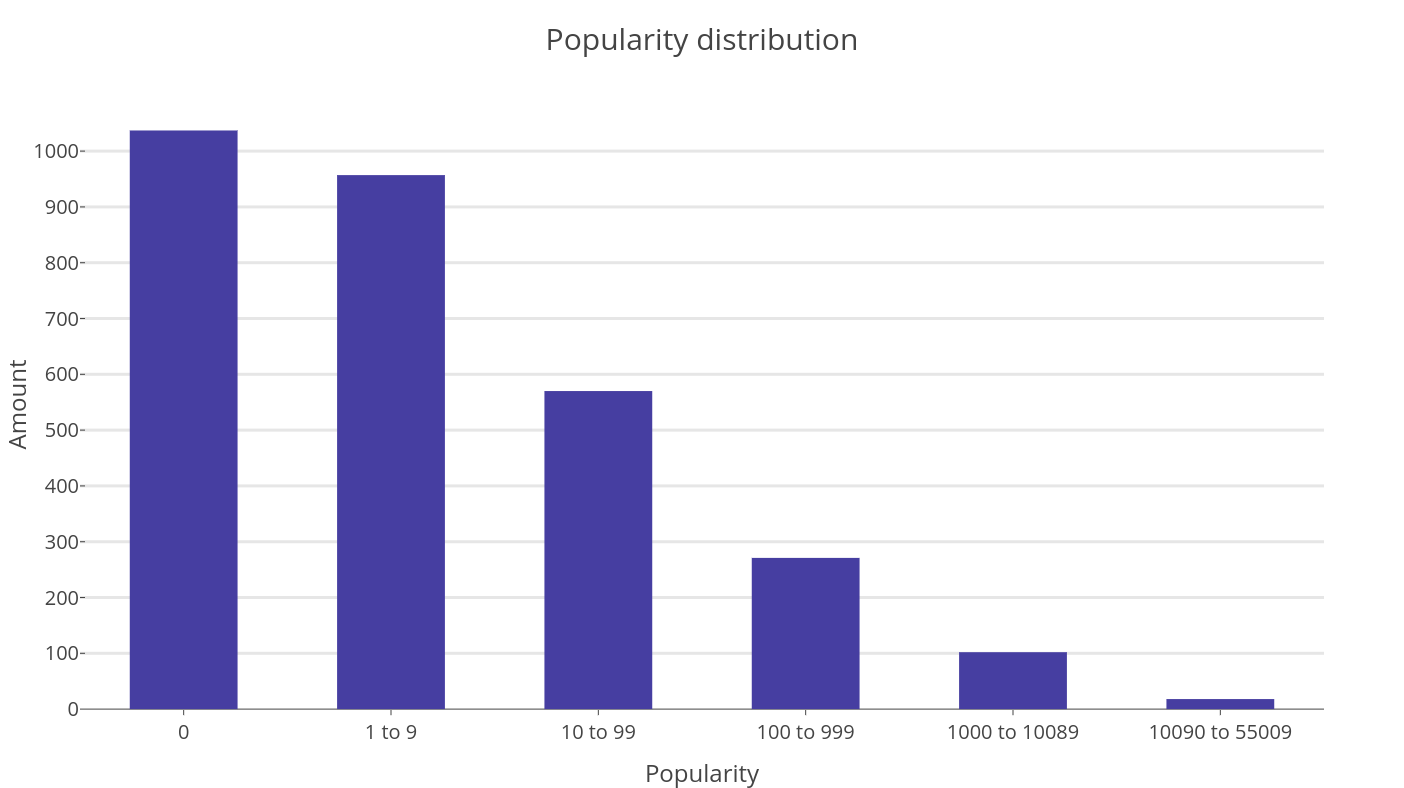
\includegraphics[width=\columnwidth]{graphics/popularityDistribution.png}
	\caption{Amount of seiyuu with that popularity, divided into groups for better visualization.}
	\label{fig:popularityDistribution}
	\end{center}
\end{figure}

This is something to take into account when trying to predict popularity of actors or explain it using other features. TODO ADD WHY

\begin{itemize}
	\item Mean:    289.55
	\item Median:    2.0
	\item Max:    55018
	\item Min:    0 (1037 values equal to zero)
	\item Only 120 values bigger than 1000
\end{itemize}

\subsection{Correlation with only one feature}
First approach to explaining popularity was using Pearson’s correlation. 

TODO PEARSON'S GRAPHIC

A fairly big correlation can be seen between popularity and amount of works. Since this data is biased to more modern anime we thought of trying to correlate with more recent works only. But, how recent? Last 5, 10 or 20 years? Thus correlation between popularity and works from different data frames was analyzed, Fig.~\ref{fig:correlationPopRecentWorks}.

\begin{figure}[!hbt]
	\begin{center}
	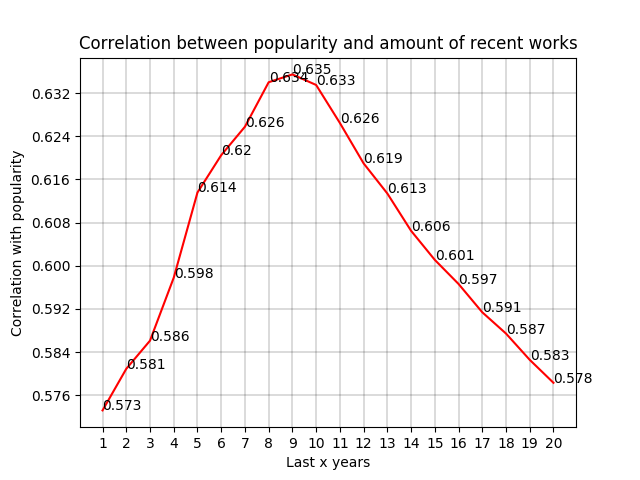
\includegraphics[width=\columnwidth]{graphics/correlationPopRecentWorks.png}
	\caption{Last \textit{X} years means works from 2018-\textit{X} to present.}
	\label{fig:correlationPopRecentWorks}
	\end{center}
\end{figure}

The best result was given by recent works from last 9 years. Therefore this definition of recent works was used from there on.

Graphics of some characteristics of works divided by years were made, trying to shed some light over why works from last 9 years were more "important". TODO EXPLANATION OF EACH FIGURE AND RE-WRITE THIS PART: 
- looking at graphs Fig.~\ref{fig:avgCaracteristicsOfWorks} it seems avg popularity, favorites and score of anime from last 9 years is not better that previous, actually is worst. but as we can see on Fig.~\ref{fig:amountOfWorksPerYear} they are more, anime industry is growing bigger each year, in a exponential way, not only that but MAL should have info of every adaptation of last year but maybe not for anime from 1980.

The majority of works are from 1990 to 2018 and half of them are distributed over the last 14 years (2014 to 2018) but as far as we can tell there isn’t anything particular over the last 9 years nor on year 2009.

\begin{figure}[!hbt]
	\begin{center}
	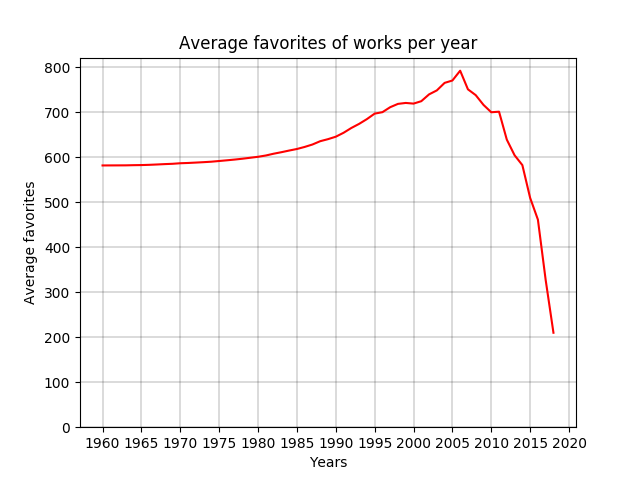
\includegraphics[width=\columnwidth]{graphics/avgFavoritesPerYear_1960-2018.png}
	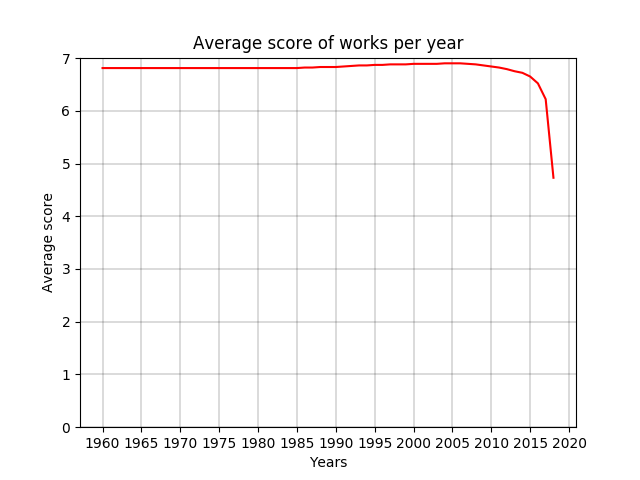
\includegraphics[width=\columnwidth]{graphics/avgScorePerYear_1960-2018.png}
	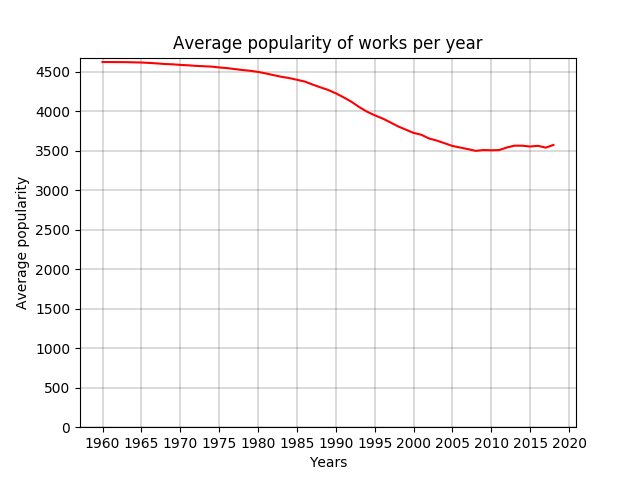
\includegraphics[width=\columnwidth]{graphics/avgWorksPopularityPerYear_1960-2018.png}
	\caption{TODO ADD DESCRIPTION.}
	\label{fig:avgCaracteristicsOfWorks}
	\end{center}
\end{figure}

\begin{figure}[!hbt]
	\begin{center}
	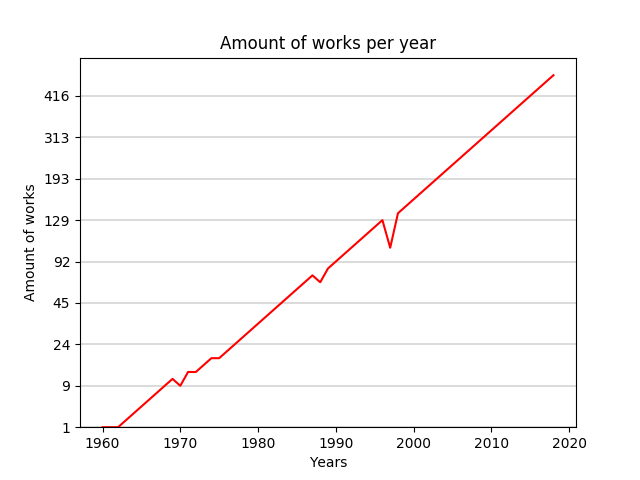
\includegraphics[width=\columnwidth]{graphics/worksPerYear_1960-2018.png}
	\caption{Amount of works divided by years which were aired for the first time.}
	\label{fig:amountOfWorksPerYear}
	\end{center}
\end{figure}

Some interesting enough correlations are shown next
TODO ADD SCATTER PLOTS AND EXPLAIN A LITTLE MORE

\subsection{Correlation with multiple features}
For this section Scikit-learn, a free software machine learning Python library, was used. The node attributes were divided into categories, leaving four distinct types:

\begin{itemize}
	\item Personal data:
	\begin{itemize}
		\item Debut
		\item Gender
		\item Activity years (2018-debut)
	\end{itemize}
	\item Works data:
	\begin{itemize}
		\item Amount
		\item Top 5 genre
		\item Favorites
		\item Score
		\item Popularity
	\end{itemize}
	\item Recent works data:
	\begin{itemize}
		\item Same as works but for only last 9 years
	\end{itemize}	
	\item Graph data:
	\begin{itemize}
		\item Degree
		\item Betweenness centrality
		\item Closeness
	\end{itemize}
\end{itemize}

Fitting and prediction experiments were run for each category, each combination of 2, 3 and all of them together; using 80\% as train data and the rest as test. This was done for all following models:
\begin{itemize}
	\item DecisionTreeRegressor
	\item DecisionTreeClassifier
	\item LinearRegression
	\item KNeighborsClassifier
	\item LinearDiscriminantAnalysis
	\item GaussianNB
	\item SVM
\end{itemize}

TODO, WRITE THIS AGAIN:
To compare prediction performance mean and median absolute error were used. Unfortunately since popularity variance is really high we observed good results in terms of absolute error but particular predictions were aloof. That's why we ended up using r2\_score for accuracy comparation. 

TODO SHOW TABLE WITH R2 SCORE RESULTS FOR EACH CATEGORY / MODEL AND GROUP OF CATEGORIES




